%!TEX root = main.tex
\chapter[PAC-Bayes Learning, a field of many paradigms]{PAC-Bayes Learning, a field of many paradigms}
\label{chap:intro-pac-bayes}

\minitoc

\addchapterlof
\addchapterloa
\addchapterloe

\section{A brief introduction to statistical learning}
\label{sec: intro-stat-learning}
Statistical learning \citep{vapnik1999overview,james2013introduction} quantifies and identifies how learning algorithms, trained on a specific task using a finite training dataset, generalise to novel, unseen datum. More precisely, an agent has to learn how to answer a question, formalised as a \emph{learning problem} being a tuple $(\H,\Z,\ell)$ composed of a \emph{predictor space} on which evolves the agent during the learning process, a \emph{data space} $\Z$ and a \emph{loss function} being the mathematical formulation of the question. Such a minimalistic structure is convenient to encompass a broad range of real-life learning scenarii. To learn, the agent has access to a \emph{training dataset} $\S_m= (\z_i)_{i=1\cdots m}$. The most classical way to learn from $\Sm$ is the empirical risk minimisation (ERM), minimising the \emph{empirical risk} $\Riskhat_{\Sm}:= \frac{1}{m} \sum_{i=1}^m \ell(h,\z_i)$. In this setting, when $\S_m$ is \iid (following the distribution $\D$), two facets of generalisation are commonly studied in statistical learning for an agent $h\in\H$.

\begin{itemize}
    \item First, the \emph{population risk} $\Risk_\D(h):= \mathbb{E}_{\z\sim\D}[\ell(h,\z)]$ focus on the average performance of our learning agent \wrt any new situation $\z\in\D$, independent of $\S_m$, possibly faced by the agent. A small population risk ensure then efficient generalisation.   
    \item Second, the \emph{generalisation gap}  $\Delta_{\Sm}(h):= \Risk_D(h) - \Riskhat_{\Sm}(h)$ evaluate the coherence between the empirical risk and the population one. Having a small generalisation gap ensure that the generalisation ability of the agent has the same magnitude than its training performance. 
\end{itemize}
Note that the population risk is a stronger notion of generalisation than the generalisation gap. However, a small generalisation gap (in absolute value) as well as a small empirical risk is enough to ensure a good population risk. Given that modern optimisation algorithm often yield small empirical risk, the generalisation gap has received a particular attention in statistical learning. 

\paragraph{Generalisation bounds.} Generalisation bounds are inequalities controlling the generalisation gap (or the population risk) by various quantities depending either on $\H,\Z$ or $\S_m$. We propose below general patterns usually involved in generalisation bounds for an agent $h_{\Sm}\in\H$ depending on $\S_m$ (for instance the output of the ERM). 

\textbf{Expected generalisation bound.} For any training set $\S_m$:

\begin{align} 
  \label{eq: expected-bound}
  \mathbb{E}_{\S_m}\LB \Delta_{\Sm}(h_{\Sm}) \RB \leq f\LP \textsc{Complexity}, \frac{1}{m}\RP. 
\end{align}

\textbf{High-probability generalisation bounds.} For any training set $\S_m$, with probability $1-\delta$ pver the draw of $\Sm$:
\begin{align}
  \label{eq: hp-bound}
  \Delta_{\Sm}(h_{\Sm}) \leq f\LP \textsc{Complexity}, \frac{1}{m}, \log\frac{1}{\delta}\RP.
\end{align}
The nature of $f$ and the \textsc{Complexity} term depend on the facet of the complexity of the learning problem we aim to focus. Celebrated examples are for instance the dimension of $\H$, if euclidean, the VC dimension of $\H$ \citep{vapnik2000learning}, the Rademacher complexity \citep{bartlett2001rademacher,bartlett2002rademacher},  the stability parameter of a learning algorithm \citep{bousquet2000algo} or the subgaussian diameter of $\Z$ \citep{kontorovich2014conc}. 
Another approach relies on the Bayesian learning paradigm, deriving \emph{posterior} knowledge from data and prior modelling of the environment. 
Then, the \textsc{Complexity} can be borrowed from information theory \citep{cover2001elements}, \eg mutual information \citep{neal2012bayesian}, or from optimal transport, \eg Wasserstein distances \citep{wang2019information,rodriguez2021tighter}. 

Those two approaches have various benefits. A notable strength of expected bounds is that they may reach fast convergence rates (\ie faster than $\frac{1}{\sqrt{m}}$) contrary to high-probability one, even when $\H$ is a singleton thanks to the central limit theorem \citep{grunwald2021mac}. However, expected bounds often involves a theoretical \textsc{Complexity} which cannot be estimated in practice and may be hard to interpret while high probability bounds may be fully empirical and can be considered with small confidence parameter $\delta$ as it is attenuated by a logarithm.

\paragraph{How to choose the complexity term ? An introductory example.} There is no evidence proving that a certain notion of complexity is preferrable to another. The choice of \textsc{Complexity} may however be driven by practical considerations, emerging from the learning problem of interest. To illustrate this point, let us focus on the following example, providing two learning problems which differs only from the predictor space $\H$ and which have very different interactions with the VC dimension.
\begin{example}[VC dimension of multilayer perceptrons]
  \label{ex: neural_net}
  Consider a supervised learning problem where $\Z = \Rbb^k\times\Ycal$ with $\Ycal=\{0,1\}$, $k$ smaller than $m$ and with loss $\ell(h,(x,y))= \mathds{1}\{h(x) \neq y\}$.  First, assume that $\Hcal$ is the set of linear classifiers; \ie $\H_1:= \left\{ h_{\theta}(x)= sgn(\langle \theta,x\rangle)  \right\}$, where $sgn(a)$ denotes the sign of $a$. In this case, using the VC dimension may lead to non-vacuous generalisation bounds \citep{vapnik2000learning}. 

However, in modern machine learning, deep neural networks are often considered, let us first define a celebrated class of deep neural networks. 

\begin{definition}[Multlilayer perceptron]
    \label{def:mlp}
    A multilayer perceptron with depth $K$ and architecture $\{N_1,\cdots,N_K\}$, denoted as $h_{\wbf}(\x) \defeq Wh^{K}(\cdots h^{1}(\x))+b$, is composed of $K$ layers $h^1(\cdot),\dots,h^K(\cdot)$.
 $W\in\R^{|\Ycal|\times N_K}$ and $b\in\R^{N_K}$ are the weight matrix and the bias of the last layer, and the $i$-th layer $h^{i}$, composed of $N_i$ nodes, is defined by $h^{i}(\xbf)\defeq\sigma_i(W_i \xbf + b_i)$, where $W_i\in\R^{N_i\times N_{i-1}}$ and the bias $b_i\in \R^{N_i}$ are its weight matrix and bias respectively; $\sigma_i : \R^{N_i} \to \R^{N_i} $ is an activation function.
The weights $\wbf=\vect(\{W, W_{K}, \dots, W_1, b, b_{K}, \dots, b_1\})$ represent the vectorisation of all parameters of the network.
\end{definition}
Now, consider the learning problem with the same $\Z,\ell$ as above, but with $\H_2$ being the set of multilayer perceptrons \wrt a fixed depth $K$ and architecture $\{N_1,\cdots,N_K\}$. To be consistent with modern practice, assume also that we are in the \emph{overparametrised setting}, meaning that the space $\H_2$ has a dimension $d$ far greater than $m$.
In this case, VC dimension fails to explain the good generalisation ability (seen in practice) of multilayer perceptrons \citep{bartlett2003vapnik}.
\end{example}

Understanding the generalisation ability of deep neural networks remains nowadays a major challenge and in what follows, we focus on a modern branch of learning theory which provided non-vacuous bounds of the generalisation ability of deep neural networks: PAC-Bayes learning.

\section{An information-theoretic exposition of PAC-Bayes learning}

PAC-Bayes learning is a recent branch of learning theory which emerged in the late 90s via the seminal work of \citep{shawe1997pac,mcallester1998some,mcallester1999pac,mcallester2003pac} and later pursued by \citep{catoni2003pac,catoni2007pac}. Modern surveys are available to describe the various advances in the field \citep{guedj2019primer,hellstrom2023generalization,alquier2024user}.  Similarly to the various subfields of statistical learning described in \Cref{sec: intro-stat-learning}, PAC-Bayes theory provide generalisation bounds involving a \textsc{Complexity} term apprehending a facet of the complexity of the learning problem. In PAC-Bayes, this term is inspired from the Bayesian learning paradigm of designing a \emph{posterior} knowledge of the learning problem based on both training data and a \emph{prior} knowledge of the considered situation. A concrete example of Bayesian learning would be an explorer mapping an ill-known territory. The explorer has to adapt the existing maps at its disposal before exploration to its discoveries. Doing so, he creates an \emph{a posteriori} map imbricating the benefits of both the prior knowledge alongside its findings. From a mathematical perspective, the Bayes approach relies on the Bayes formula, providing an update recipe from a prior distribution $\P\in\Mcal(\Hcal)$ over the predictor space $\H$ to a posterior $\Q\in\Mcal(\Hcal)$ through a likelihood. On the contrary, PAC-Bayes, while inspired from the Bayesian philosophy, does not relies on the Bayes formula but instead on tools from information theory. This general approach benefits from additional flexibility as PAC-Bayes can be linked and applied to Bayesian learning (see \citealp{guedj2019primer}) but also blurs the notion of prior and posterior distributions, now independent of the fundamental Bayes formula. We further develop those points through two celebrated  high-probability bounds: the McAllester and Catoni ones. 

\subsection*{Two fundamental results}
    The McAllester's bound \citep{mcallester2003pac} enriched with Maurer's trick \citep{maurer2004note} and Catoni's bound (\citealp[Theorem 4.1]{alquier2016properties}, being a relaxation of \citealp[Theorem 1.2.6]{catoni2007pac}) are probably the most known high-probability PAC-Bayes bounds. We recall them in \Cref{prop: mcall-catoni}.

    \begin{proposition}[McAllester and Catoni's bounds]
        \label{prop: mcall-catoni}
        Assume $\Sm$ to be \iid.\\
    \textbf{McAllester's bound, \citep[Theorem 5]{maurer2004note}.}  For any $\delta\in(0,1),\ell\in[0,1]$, any data-free prior $\P\in\Mcal(\Hcal)$, with probability at least $1-\delta$, for any posterior $\Q\in\Mcal(\H)$,
    \begin{align}
    \label{eq: mcallester}
     \Delta_{\Sm}(\Q) \le \sqrt{\frac{\KL(\Q,\P) + \ln{\frac{2\sqrt{m}}{\delta}}}{2m}}.
    \end{align}

    \textbf{Catoni's bound, \citep[Theorem 4.1]{alquier2016properties}.}
    For any $\lambda\in\mathbb{R}/\{0\},\delta\in(0,1),\ell$ being $\sigma^2$-subgaussian and a data-free prior $\P$, with probability at least $1-\delta$ over $\S$, for any $\Q\in \Mcal(\Hcal)$,

  \begin{align}
    \label{eq: catoni}
    \Delta_{\Sm}(\Q) \leq  \frac{\KL(\Q,\P) + \log(1/\delta)}{\lambda} + \frac{\lambda\sigma^2}{2m}.  
  \end{align}

    For both results, $\Delta_{\Sm}(\Q)$ denotes the expected generalisation gap \wrt $\Q$ and $\KL$ denotes the Kullback-Leibler divergence.
    \end{proposition}

Recall that a random variable $X$ is $\sigma^2$-subgaussian if for any $\lambda\in\Rbb$, $\Ebb[\exp(\lambda(X-\Ebb[X]))] \leq \exp\LP \frac{\lambda^2 \sigma^2}{2} \RP$ and that any loss $\loss\in[0,C]$ is $C$-subgaussian. Both McAllester and Catoni bounds fit the general shape of \eqref{eq: hp-bound}. In both cases, $\textsc{Complexity}= \KL(\Q,\P)$ and $f$ varies. The immediate link with the Bayesian philosophy of learning is that the prior has to be data-free. However, \eqref{eq: mcallester} and \eqref{eq: catoni} are both valid simultaneously for any posterior, which is strictly more general than considering the Bayesian posterior. Note that if $\lambda$ is optimised, then Catoni's bound would boil down to an upgraded McAllester bound without the $\log(\sqrt{m})$ term, but such an optimisation is not feasible as $\lambda$ has to be chosen independently of the dataset $\Sm$. 
Note that this gap has been recently filled by \citet[Theorem 33]{dupuis2024generalization}. While the theoretical links between those two bounds are clear, they involve two different toolboxes: McAllester's bound heavily relies on the KL divergence between Bernoullis alongisde calculation tricks exploiting the boundedness of the loss while the original Catoni's bound \citep[Theorem 1.2.6]{catoni2007pac} exploits tools from statistical physics. 
The relaxation \eqref{eq: catoni} proposed here is reachable by a few key arguments, involved in a vast majority of PAC-Bayes proofs. We propose it below for pedagogical purpose. 

\begin{proof}[of \Cref{eq: catoni}]
Note that the first part of the proof holds for a large part of PAC-Bayes literature.

  \textbf{A generic pattern for PAC-Bayes bounds.}
    This part is designed upon two cornerstones, retrievable in many existing results: the change of measure inequality (\citealp{csizar1975divergence,donsker1976asymp} -- see also \citealp{banerjee2006bayesian,guedj2019primer} for a proof) and Markov's inequality.

  \begin{lemma}[Change of measure inequality]
    \label{l: change_meas} 
    For any measurable function $\psi :\mathcal{H}\rightarrow \mathbb{R}$ and any distributions $\Q,\P$ on $\mathcal{H}$:
    
    \[ \mathbb{E}_{h\sim \Q}[\psi (h)] \leq \operatorname{KL}(\Q,\P) + \log\left( \mathbb{E}_{h\sim \P}[\exp(\psi(h))]  \right).  \]
    \end{lemma}
For a given $\lambda>0$, the change of measure inequality is then applied to a certain function $f_m: \Hcal \rightarrow\mathbb{R}$, possibly involving $\Sm$: for all posteriors $Q$,
\begin{align}
\label{eq: change_meas_pacb}
\mathbb{E}_{h\sim \Q}[f_m(h)] \leq \operatorname{KL}(\Q,\P) + \log\left( \mathbb{E}_{h\sim \P}[\exp(f_m(h))]  \right).
\end{align}
To deal with the random variable  $X(\Sm):=\mathbb{E}_{h\sim \P}[\exp(f_m(h))] $, our second building block is Markov's inequality $\left(\mathbb{P}(X>a) \leq \frac{\mathbb{E}[X]}{a}\right)$ which we apply for a fixed $\delta\in (0,1)$ on $X(\Sm)$ with $a= \mathbb{E}_{\Sm}[X(\Sm)]/\delta$.
Taking the complementary event gives that for any $m$, with probability at least $1-\delta$ over the sample $\Sm$, $X(\Sm)\leq \mathbb{E}_{\Sm}[X(\Sm)]/\delta$, thus:


\begin{equation}
  \label{eq: prelim_pb_bound}
  \mathbb{E}_{h\sim \Q}[f_m(h)] \leq \operatorname{KL}(\Q,\P) + \log(1/\delta) + \log\left( \mathbb{E}_{h\sim P}\mathbb{E}_{\Sm}[\exp(f_m(h))]  \right).
\end{equation}

Note that in \eqref{eq: prelim_pb_bound}, we swapped the two expectations in the last term thanks to Fubini's theorem and the fact that $\P$ is data-free.

\textbf{Proving Catoni's bound.}
Now, we take $f_m(h)= \lambda\Delta_{\Sm}$ and consider for any $h\in\Hcal, A(h)= \mathbb{E}_{\Sm}[\exp(f_m(h))]$. 

Note that, given $\Sm$ is iid, 
\begin{align*}
  A(h) &= \prod_{i=1}^m \mathbb{E}_{\Sm}\LB\exp\LP\frac{\lambda}{m}(\Risk_\D(h)-\ell(h,\z_i))\RP\RB, 
  \intertext{and thanks to Heoffding's lemma alongside $\ell$ being $\sigma^2$-subgaussian,}
  A(h) &\leq \prod_{i=1}^m \exp\LP \frac{\lambda^2 \sigma^2}{2m^2} \RP = \exp\LP \frac{\lambda^2 \sigma^2}{2m} \RP.
\end{align*}

Plugging this upper bound in \eqref{eq: prelim_pb_bound} and dividing by $\lambda$ concludes the proof.
\end{proof}

The generic pattern \eqref{eq: prelim_pb_bound}, allows to retrieve many PAC-Bayes bounds, starting with McAllester's one, where $f_m= kl(\Risk_\D(h),\Riskhat_{\Sm}(h)), kl$ being the KL divergence between Bernoullis and completing with the subtle calculations of \citet{maurer2004note}. This pattern is also valid, for instance, for the results of \citet{germain2009pac}, the Bernstein PAC-Bayesian bounds of \citet{tolstikhin2013pac,mhammedi2019pac} and many other results, \eg \citet{thiemann2017strongly,guedj2018pac,holland2019pac,wu2022split}. This then pins two major points for a large part of PAC-Bayes literature: 

\begin{enumerate}
  \item Interpreting PAC-Bayes from a Bayesian point of view is legitimated by the change of measure inequality, yet the KL divergence. More generally, this property allows interpreting PAC-Bayes under a more general information-theoretic paradigm, where relevant prior information is transferred to the posterior (here by absolute continuity to keep the KL finite). This information-theoretic vision is also retrieved in in-expectation PAC-Bayes bounds, where mutual information can be considered instead of KL divergence \citep{russo2016control,xu2017info,steinke2020reason,grunwald2021mac,hellstrom2020gene,hellstrom2022new}. 
  \item The statistical properties of the learning problem are linked to the exponential moment coming from the change of measure inequality, this often implies the strong assumptions of \Cref{prop: mcall-catoni}: data-free prior, bounded or subgaussian losses (sometimes attenuated to subexponentiality \citealp{catoni2004statistical}).
\end{enumerate}

\paragraph{A theory suited for \Cref{ex: neural_net}?}
The two previous points show that \Cref{prop: mcall-catoni} holds for learning problem with light-tailed losses (often bounded), \iid data, encompassing classification tasks for instance. Then, PAC-Bayes learning seems suited to understand, on such problems, the McAllester and Catoni bounds are suited to the learning problem $(\Hcal_2,\Z,\ell)$ of \Cref{ex: neural_net}. 

However, the question of their tightness is unsolved as we do not know the behavior of the KL term in practice. Furthermore the question of which distribution $\Q$ should be taken in \Cref{prop: mcall-catoni} remains open. Hopefully, PAC-Bayes bounds can be transformed into learning algorithms.

% Rework this paragraph, do not talk about dziugaite now, just say that the  theoretical framework fits the learning problem of example 1.1.1. But it still needs to be verified that this complexity measure will be small for neural nets, and thus, non-vacuous bound can be attained in this case.

\section{From theory to learning algorithms}

\subsection*{Algorithms associated to McAllester and Catoni bounds}
A shared particularity of McAllester and Catoni bounds is that they are both fully empirical. Then it is possible to minimise them in practice and thus, deriving new theory-driven learning algorithms which are expected to have at worse, a small generalisation gap and at best, a small population risk. More precisely, learning algorithms associated to \Cref{prop: mcall-catoni} are stated below: 

\begin{align}
  \label{eq: alg-mcall}
  \Q_{M}:= \underset{\Q\in\mathcal{C}}{\operatorname{argmin}}\; \Riskhat_{\Sm}(\Q) + \sqrt{\frac{\KL(\Q,\P)}{2m}}.
  \intertext{For any $\lambda>0$,}
  \label{eq: alg-catoni}
  \Q_{C}:= \underset{\Q\in\mathcal{C}}{\operatorname{argmin}}\; \Riskhat_{\Sm}(\Q) +\frac{\KL(\Q,\P)}{\lambda}.
\end{align}
In both cases, $\mathcal{C}\subseteq \Mcal(\Hcal)$ is the class of distributions on which we optimise. The choice of $\mathcal{C}$ can come from a priori knowledge of the problem or from optimisation concerns to make the KL divergence tractable.  

Knowing Catoni's bound is a relaxation of McAllester's one, it seems more natural to consider $\Q_{M}$ over $\Q_{C}$. However, the presence of a square root in \eqref{eq: alg-mcall} can be challenging for practical optimisation. We illustrate this below.
\begin{example}[A celebrated class of measures for PAC-Bayes algorithms]
  \label{ex: gaussian-kl}
  Consider the case where, for a given $\sigma>0$, $\mathcal{C}= \{\Ncal(\mu,\sigma^2 \mathrm{Id}) \mid \mu\in\Rbb^d\}$. Then the for any $\P= \Ncal(\mu_1,\sigma^2 \mathrm{Id}), \Q= \Ncal(\mu_2,\sigma^2 \mathrm{Id})$, $ \KL(\Q,\P)= \frac{\|\mu_1-\mu_2\|^2}{2\sigma^2}$. 
  Then, optimising \eqref{eq: alg-mcall} in this case implies to lose the strong convexity of the KL divergence while it is retained for \eqref{eq: alg-catoni}.
\end{example}
  
Another practical advantage of \eqref{eq: alg-catoni} over \eqref{eq: alg-mcall} emerges when $\mathcal{C}= \Mcal(\Hcal)$. In this case, Catoni's bound admits a closed form solution, while McAllester's one should be numerically optimised on all the space of distributions, which is not feasible. This closed form, extracted from \citet[Section 5.1]{catoni2003pac}, is recalled below.

\begin{align}
  \label{eq: catoni-gibbs}
  \text{When}\; \mathcal{C}= \Mcal(\Hcal),\; d\Q_{C}(h) = \frac{\exp(-\lambda \Riskhat_{\Sm}(h))}{\Ebb_{h\sim\P}[\exp(-\lambda \Riskhat_{\Sm}(h))]} d\P(h)
\end{align}

Then, $\Q_{C} = \P_{-\lambda \Riskhat_{\Sm}}$ is the \emph{Gibbs posterior} associated to $\P,\lambda\Riskhat_{\Sm}$. By introducing Gibbs posterior in statistical learning, \citet{catoni2007pac} draws a theoretical link between statistical physics and learning theory. Unfortunately, Gibbs posteriors often require Monte Carlo methods to be implemented, which can be time-consuming. Below, we then focus on PAC-Bayes algorithms working on a subset $\mathcal{C}$ of $\Mcal(\Hcal)$. 

\subsection*{Instantiation and efficiency of PAC-Bayesian algorithms}

\paragraph{A general pattern for PAC-Bayesian algorithms}

The introductory examples \eqref{eq: alg-mcall},\eqref{eq: alg-catoni} unveil a general design for any KL-based PAC-Bayesian algorithm, satisfying a trade-off between \textit{(i)} the empirical risk, showing that the learner has to fit the training dataset, and \textit{(ii)} a \emph{regulariser} being a function of $\KL(\Q,\P)$. This regulariser ensures that, during training, the learner will not overfit on training data. This training ensures a good generalisation ability as long as the associated generalisation bound is small. 

While the conceptual ins and outs of PAC-Bayes algorithms are getting clearer, two unanswered questions remains: 

\begin{enumerate}
  \item How are those algorithms instantiated in practice?
  \item Are these algorithms efficient and do they come with non-vacuous theoretical guarantees? 
\end{enumerate}

\paragraph{Instantiating a PAC-Bayes algorithm}
  In practice, using a single prior $\P$ usually does not work, but it remains theoretically possible to consider a finite set of priors. Indeed, if one wants to consider $k$ priors, then it is possible to consider $k$ PAC-Bayes bounds holding for each of those priors with probability at least $1-\frac{\delta}{k}$ and then consider a union bound, such a set of priors is called a grid. This method has been widely used in many PAC-Bayes work with clever grids, deteriorating initial bounds at the cost of supplementary $\log(n)$ or $\log\log(n)$ (divided by $m$), see \eg \citet{alquier2024user}. 
  This can also be used, for Catoni-typed algorithms, to the parameter $\lambda$. In both cases, considering grids allows to optimise on both the prior, the posterior (and possibly $\lambda$ when involved) and then taking the closest value of those optimised parameters on the grid to still obtain theoretical guarantees. Another technique to ensure a good prior is to sacrifice a part of the training set to pre-train $\P$. 
  Doing so, the prior is then data-dependent and yields tighter bounds alongside increased performance \citep{perez2021tighter,perezortiz2021learning}.

\paragraph{Efficiency of PAC-Bayes algorithms on supervised learning problems.}
The work of \citet{dziugaite2017computing} showed that optimising \eqref{eq: alg-mcall} when $\mathcal{C}$ is a class of Gaussian measures for the weights of a deep neural network yields non-vacuous generalisation bound, meaning that the generalisation benefits of PAC-Bayesian training on deep nets can be theoretically ensured. Note that PAC-Bayesian bounds can also be used to quantify the generalisation ability of other learning algorithms, but the bound value is then suboptimal.  \citet{dziugaite2017computing} used the toolbox described in the 'instantiation' paragraph, alongside a preliminary use of Stochastic Gradient Descent (SGD) to update $\Q$ before the PAC-Bayes training algorithm. This promising work paved the way to various extensions, providing non-vacuous guarantees for a wide range PAC-Bayes algorithms \citep{rivasplata2019pac,letarte2019dichotomize,perezortiz2021learning,perez2021progress,perez2021tighter,dziugaite2021role,biggs2022non,biggs2023tighter}, showing that the PAC-Bayes toolbox provides elements of answer to understand the generalisation ability of neural networks. Beyond generalisation guarantees, PAC-Bayes bounds are also useful to propose original training methods, even if the associated guarantees are vacuous \citep{biggs2021differentiable,biggs2022margin}. Another important empirical use is to exploit PAC-Bayes bounds as correlation measures, to see whether a decrease of the bound is related to an increased generalisation ability of the learner. For instance \citet{neyshabur2017explor} used McAllester's bound \eqref{eq: mcallester} as a 'flatness' measure and showed that it correlates well with a good generalisation ability for a few learning problems. This conclusion has been extended to a wider range of problems in \citet{jiang2020fantastic,dziugaite2020search}. 

\paragraph{PAC-Bayes algorithms beyond supervised learning.} While supervised learning is a widely used to perform experiments in PAC-Bayes (often involving celebrated datasets such as MNIST or CIFAR-10), the McAllester bound holds for any learning problem with bounded loss, going beyond this setting. This theoretical flexibility has been exploited to derive PAC-Bayesian algorithm for various learning settings reinforcement learning \citep{fard2010pac}, multi-armed bandits \citep{seldin2011pac,seldin2012pac,sakhi2023pac}, meta-learning \citep{amit2018meta,farid2021generalization,rothfuss2021pacoh,rothfuss2022pac,ding2021bridging} to name but a few. 

\paragraph{Is \Cref{ex: neural_net} tackled now?}
\citep{dziugaite2017computing} and following works have provided a positive answer by obtaining non-vacuous guarantees (sometimes tight) for $(\Hcal_2,\Zcal,\ell)$ of \Cref{ex: neural_net} for various $\Z$ (being, \eg, set of images for MNIST CIFAR-10 etc...). To obtain such guarantees, a PAC-Bayesian training needs to be performed to minimise its associated theoretical bound. That being said, several questions then legitimately emerge.

\begin{itemize}
  \item Modern machine learning often implies learning problems where assumptions such as bounded (or subgaussian) losses or \iid data do not hold. Is PAC-Bayes theory extendable beyond those assumptions? 
  \item As shown in \citet{dziugaite2017computing}, the PAC-Bayesian training is often combined to another procedure (\eg ERM) to yield non-vacuous bounds. However, PAC-Bayes bounds do not bring the theoretical understanding of such additional methods, often outputting deterministic predictors (\ie Dirac distributions). This kind of predictor is not allowed in \eqref{eq: mcallester}, \eqref{eq: catoni}. Is it possible to obtain PAC-Bayes bounds valid for such methods? 
\end{itemize}



\section{An optimisation perspective of PAC-Bayes}

The questions raised at the end of the previous part are important as they underline a gap between the information-theoretic approach of PAC-Bayes bounds and practical optimisation. A supplementary example of this is the grid required in practice to optimise the prior (and/or $\lambda$ in Catoni's bound). Indeed this hybrid solution is required to roughly fit theory,(exploiting a single prior) and practice (optimising freely the prior on a continuous space), while not being truly adapted to any of these settings. This then raises the following fundamental question:
\[ \textbf{Can we think PAC-Bayes learning from an optimisation perspective?} \]

The elements of answer to this question are multiple. First, one can mix PAC-Bayes argument with geometric properties of optimisation procedure to obtain generalisation bounds designed for specific algorithms exploiting their geometric properties and assumptions, including but not limited to, SGD, Langevin dynamics  \citep{london2017pac,dziugaite2018entropy,neu2021info,clerico2022generalisation,haghifam2023limit,zhou2023toward}. Those works shows both convergence properties as well as minimax rates, showing the impact of PAC-Bayes learning to provide a better theoretical understanding of the generalisation ability of concrete algorithms. 

A second approach consists in describe general principles that should be satisfied by the various terms and assumptions in PAC-Bayes when looking at this through the prism of optimisation. We propose such an analysis below.

\subsubsection*{An optimisation-driven view of PAC-Bayes}

\begin{itemize}
  \item \textbf{Statistical assumptions.} While $\ell$ satisfies desirable geometric properties (convexity, gradient lipschitz ...), no statistical assumption is needed to have optimisation algorithms with convergence properties, on then may wonder about the generalisation abilities of the reached empirical minima. It happens that the output of two runs of a stochastic optimisation algorithm on the same training set may vary a lot, for instance, the specific case of SGD shows that  heavy-tailed behaviour (see \eg \citealp{simsekli2019tail,zhang2020adaptive,gurbuzbalaban2020heavy}) may emerge in practice. Given such behaviours, generalisation bounds, from an optimisation point of view, should hold with weak statistical assumptions on the dataset, possibly at the cost of additional geometric assumptions on the loss.
  \item \textbf{The role of the prior.} The information-theoretic approach justifies the Bayesian view of the prior, as discussed earlier. In this spirit it is also possible to sacrifice a part of the training set (\ie of the available information) to enrich $\P$. Doing so, we accept to not understand what happens during the training of $\P$ and thus, to explain partially the efficiency of an information-theoretic training. Those two visions (Bayesian prior or data-dependent prior) are not easily linked to optimisation concerns as the first one would be linked to a 'good' initialisation, something we cannot know in advance, while the second makes little sense as $\P$ is obtained through a first, unexplained, optimisation process which is necessary to understand the efficiency of the second part of training, outputting $\Q$. From an optimisation stance, we suggest to assign only two possible roles to $\P$: \textit{(i)} the initialisation of the optimisation algorithm, then its impact should be attenuated through the learning process and \textit{(ii)} a minimiser we aim to reach through optimisation. In this case, its impact is crucial as it translates the speed of convergence of our learning algorithms.
  \item \textbf{The place of stochastic predictors.} Involving a KL divergence as a complexity brings a particular focus on stochastic predictors, drawn from a distribution $\Q$. Classical PAC-Bayes bounds usually focus on the average performance of such a predictor (hence the expectation over $\Q$ in \eqref{eq: mcallester},\eqref{eq: catoni}), but recent extensions directly proposed guarantees for a single draw over $\Q$ \citep{rivasplata2020pac,viallard2023general}. However, involving a KL implies that $\Q$ has to be absolutely continuous \wrt $\P$,  meaning that the support of $\Q$ cannot go beyond the one of $\P$: this excludes the case of Dirac distributions, \ie deterministic predictors. This is a clear limitation of the information-theoretic approach, as many learning algorithms outputs a deterministic predictor and thus, should be avoided to be in line with common practice in optimisation.
\end{itemize}

Those three points, while not necessarily considered explicitly through the lens of optimisation have been recently challenged.



\subsubsection*{PAC-Bayes beyond the usual setting}

Recall that according to what we saw in McAllester's bound \eqref{eq: mcallester} and Catoni's one \eqref{eq: catoni}, we denote by usual setting a bound holding for \iid $\Sm$, with bounded or subgaussian losses and involving a KL divergence as \textsc{Complexity} term. Many works overcame at least one of this assumption as precised below. 

\paragraph{Beyond \iid data} The work of \citet{fard2010pac} established links between reinforcement learning and PAC-Bayes theory. This naturally led to the study of PAC-Bayesian bound for martingales instead of \iid data \citep{seldin2011pac,seldin2012bandit,seldin2012pac}. Also, PAC-Bayesian bound for lifelong learning \citep{pentina2014pac,flynn2022pac} challenged also the \iid assumption. We also denote that the PAC-Bayes bound for meta learning \citep{amit2018meta,farid2021generalization,rothfuss2021pacoh,rothfuss2022pac,ding2021bridging} consider independent but non-identically distributed datasets (corresponding to different tasks).

\paragraph{Avoiding light-tailed losses.} Light-tailed losses encompass bounded, subgaussian, subexponential losses. Deriving PAC-Bayes bound for heavy-tailed losses, starting from \citet{audibert2011robust} which provided PAC-Bayes bounds for least square estimators with heavy-tailed random variables. Their results was suboptimal with respect to the intrinsic dimension and was followed by further works from \citet{catoni2016pac} and \citet{catoni2017dimension}.
More recently, this question has been addressed in the works of \citet{alquier2018simpler, holland2019pac,kuzborskij2019efron,haddouche2021pac}, extending PAC-Bayes to heavy-tailed losses under additional technical assumptions.

\paragraph{Towards data-dependent priors.} The work of \citep{catoni2007pac,lever2010distribution,lever2013tighter} proposed priors, not directly data-dependent, but depending of the data distribution $\Dcal$ when \iid data are considered. can be informed by the
data-generating distribution, \citet{parradohernandez2012pac,oneto2016pac,dziugaite2017computing,mhammedi2019pac} also obtained PAC-Bayes bound with data-dependent priors by infusing directly data in the prior (and sacrificing a part of the dataset). The drawback of this method is that, in practice, such a prior allows tighter bounds, but at the cost of a reduced theoretical understanding as the prior is in practice often learned via ERM, and the PAC-Bayes bound hardly gives insights on what happens during this pre-training. Furthermore, if this pre-training has already made the bound converge to a minimum generalising well, then the PAC-Bayes training has no effect and the associated bound is no more than a test bound (the case $\Q=\P$). It has been shown for instance in \citep{perezortiz2021learning} that when $\P$ is trained with a consequent fraction of data, then the generalisation performance of the pre-trained $\P$ was roughly the same than $\Q$, obtained from $\P$ after a PAC-Bayesian training. It is then unclear how impacting are PAC-Bayes methods compared to a test bound in this case. To alleviate this issue, another original route \citep{dziugaite2018data} exploits differential privacy to replace the data-free prior by a differentially private one, making possible to consider the prior as the learning objective (in their case a Gibbs posterior).

\paragraph{Beyond KL divergence.} Several works allowed to extend PAC-Bayes beyond KL divergences. The most investigated route is to focus on the more general class of $f$-divergence, which include, \eg, KL, $\chi^2$, Rényi divergences among others \citep{alquier2018simpler,ohnishi2021novel,picard2022change,viallard2023general}. However, $f$-divergences still implies absolute continuity of $\Q$ \wrt $\P$. Another route recently emerged \citep{amit2022integral}, replacing $f$-divergences by integral probability metrics (IPMs), finally allowing Dirac distribution in PAC-Bayes.


These works have sometimes been explicitly driven by optimisation considerations (\citealp{dziugaite2018data} involved differential privacy to numerically tighten their bound without sacrificing data). However, in many cases, the information-theoretic vision of PAC-Bayes remained majoritary. In what follows, the contributions of this manuscript are designed \wrt the optimisation view of PAC-Bayes detailed above. 

\subsubsection*{Contributions of this thesis}

The contributions of this manuscript are motivated by optimisation considerations and are structured as follows: 

\begin{itemize}
  \item In Chapter 2, we propose novel PAC-Bayes bounds for martingales, batch learning, with an application to multi-armed bandits. Those bounds are anytime-valid (\ie for any dataset size simultaneously) and holds at the sole assumption of finite order 2 moments on both the posterior and the data distribution. Such weak statistical assumptions make these results applicable, for instance, for heavy-tailed SGD or many learning problems where optimisation procedure are performed regardless of the training set noise.
  \item Chapter 3 introduces \emph{Online PAC-Bayes learning}, proposing theoretical bounds and learning algorithms involving a sequence of pairs $(\Q_i,\P_i)$, evolving through the optimisation process. Contrary to PAC-Bayes in a batch setting, the impact of $\P=\P_1$ is attenuated during the learning process, making Online PAC-Bayes useful when there is no prior information available, which is consistent with the vision of $\P$ as initialisation of a learning algorithm, while being only applicable, for now, to stochastic predictors as a KL divergence is involved.
  \item Chapter 4 still consider the prior as an initialisation point, but this time, considering batch learning algorithms. It is shown that the impact of the prior is attenuated by \emph{flat minima}, \ie minima such that their neighbourhood nearly minimises the loss. More generally, this chapter exhibits theoretical links between flat minima and generalisation and thus draw links between the benefits of a successful optimisation process (small gradients) and generalisation.
  \item Considering $\P$ as the learning objective allows to draw more explicit links between optimisation and generalisation. In Chapter 5, it is shown that the convergence guarantees of \emph{Bures-Wasserstein SGD}, a SGD-like algorithm on Gaussian measure spaces, can be directly incorporated within PAC-Bayes bounds, yielding interpretable results. This is possible by exploiting \emph{Wasserstein PAC-Bayes learning}, which uses as \textsc{Complexity} term a 1-Wasserstein distance, allowing to trade statistical assumptions to geometric ones such as lipschtz or gradient-lipschitz losses. 
  \item Wasserstein PAC-Bayes learning can also be exploited when $\P$ is seen as an initialisation point. In Chapter 6, we propose Wasserstein PAC-Bayes algorithms with associated theoretical bound for both batch and online learning. A notable strength of these methods is that they hold for deterministic predictors (Dirac distributions), making PAC-Bayes in line with a large part of optimisation algorithms.
\end{itemize}

To conclude this introduction we recap in \Cref{fig: recap-info,fig: recap-optim} the classical information-theoretic vision of PAC-Bayes alongside the original optimisation view proposed above. 

\begin{figure}[ht]
  \centering
  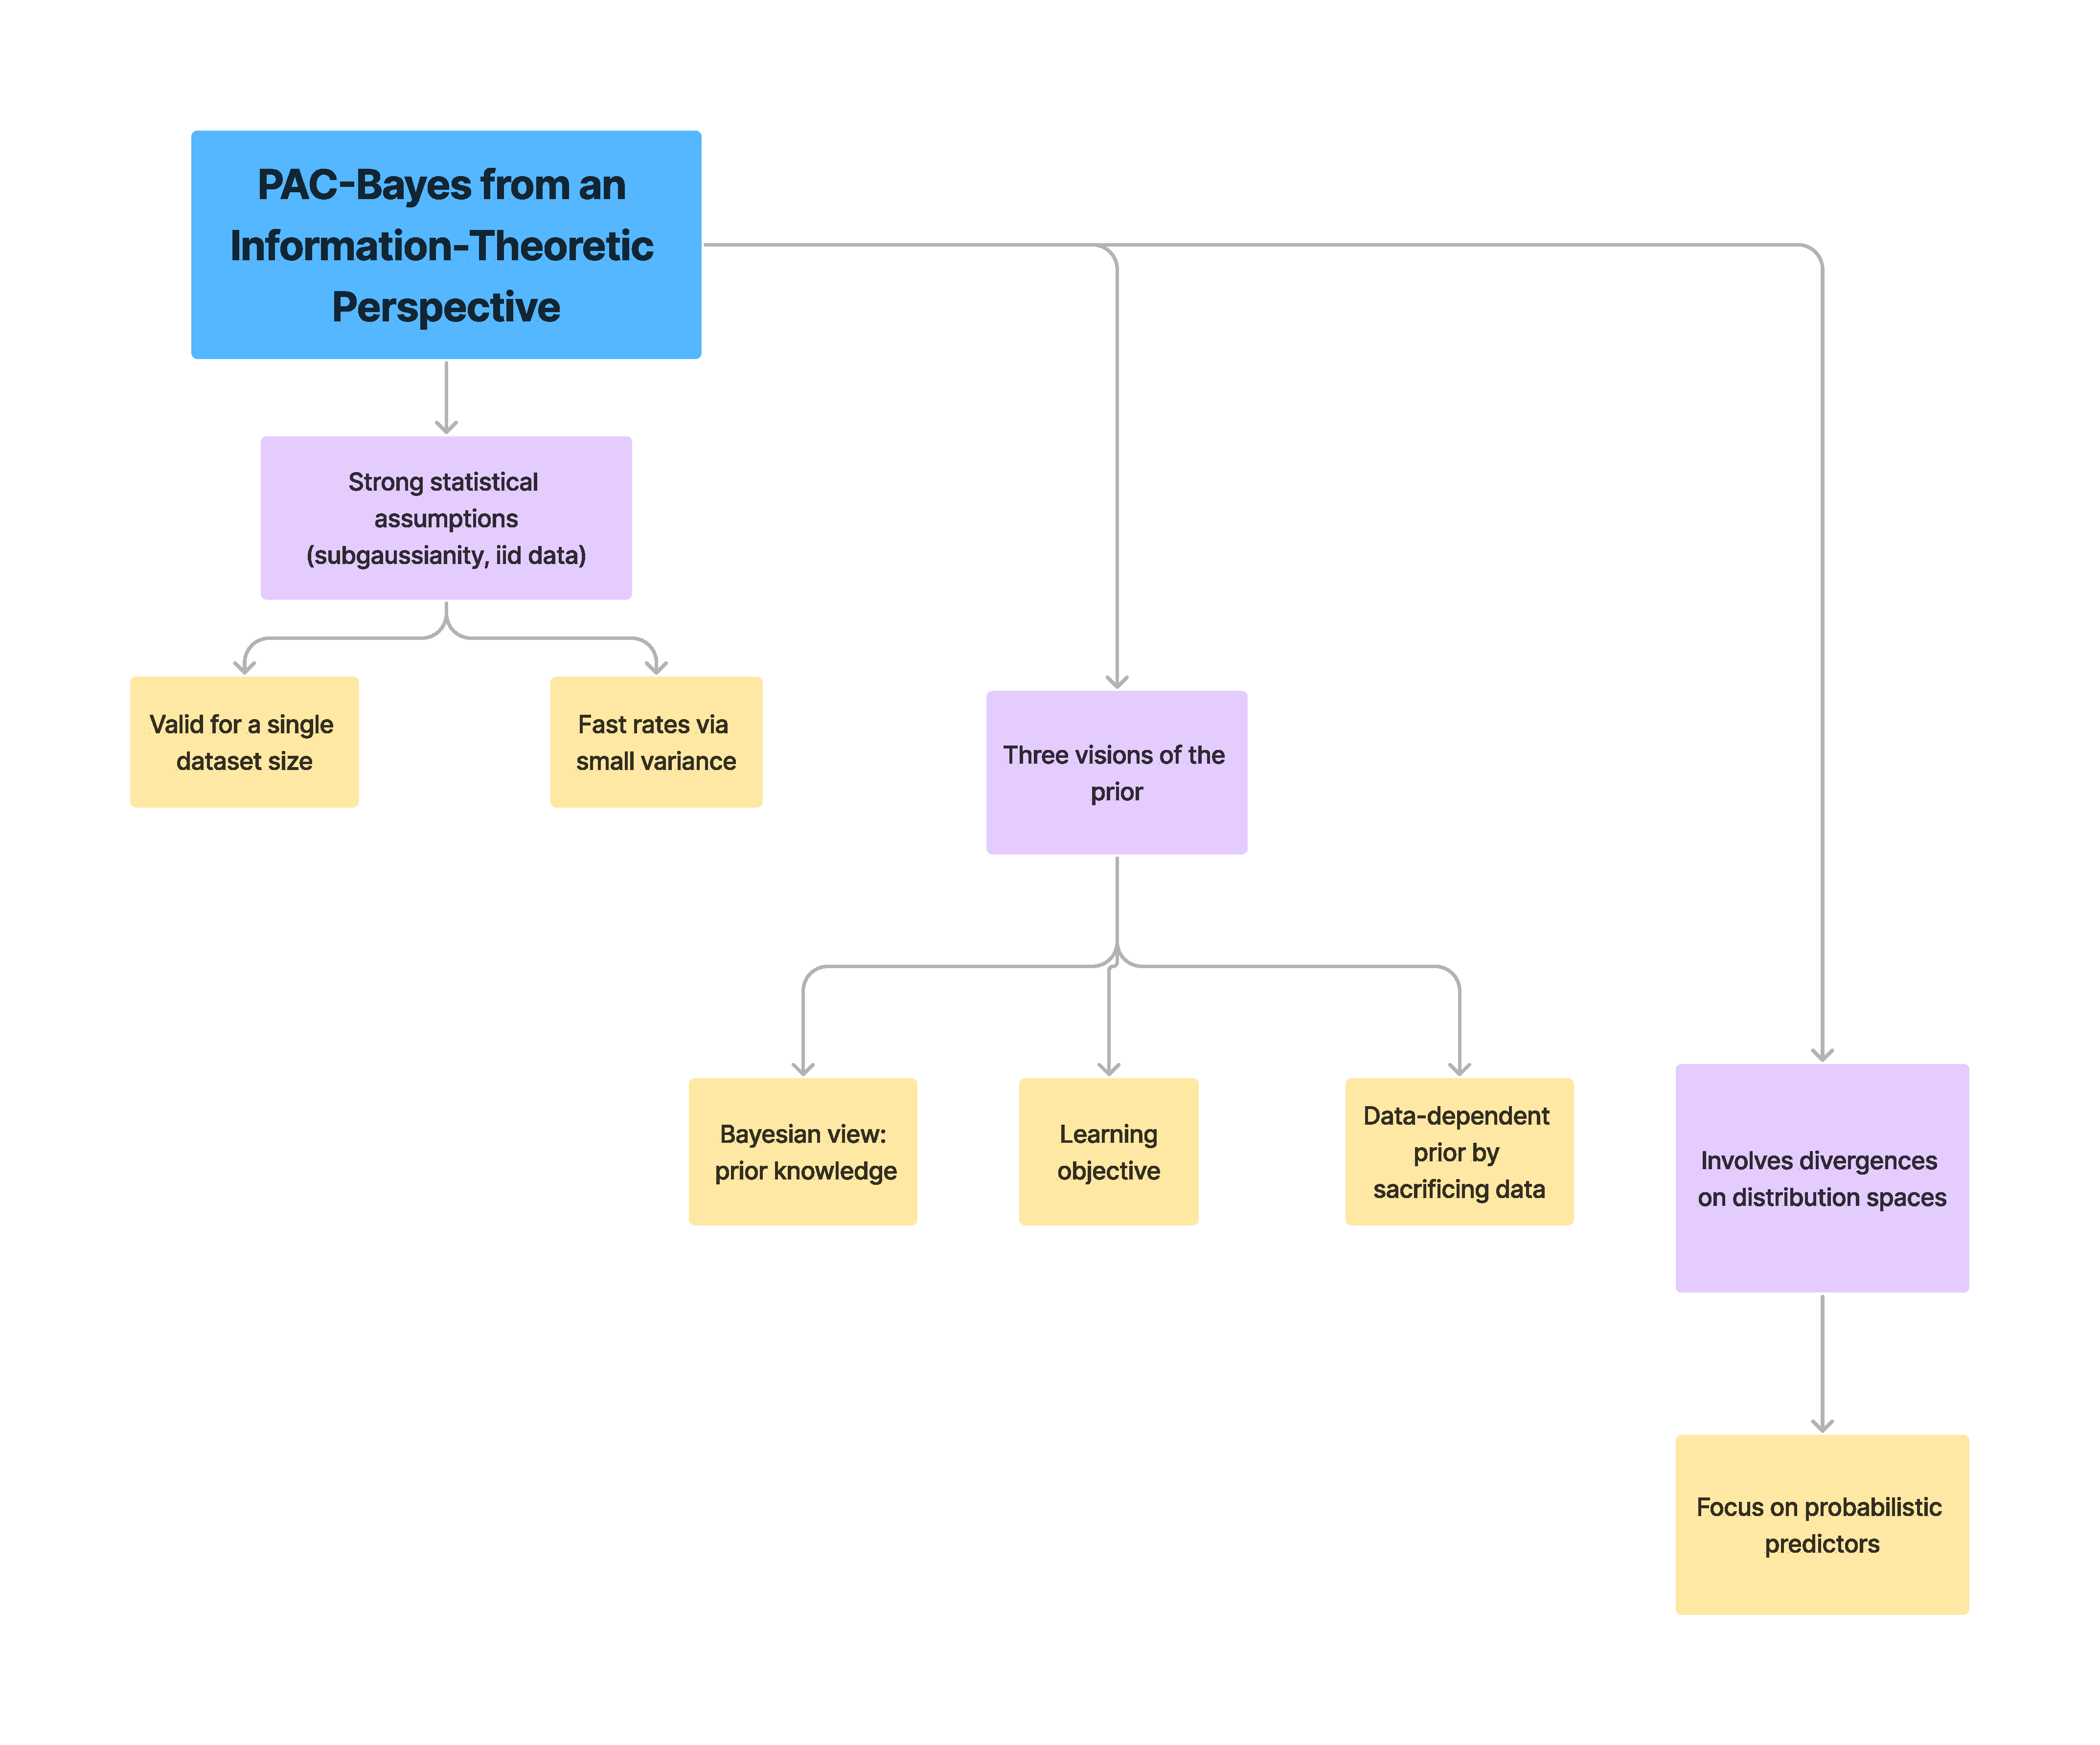
\includegraphics[width=1.0\linewidth]{chapter_1/recap-info.pdf}
  \caption{Recap of the information-theoretic vision of PAC-Bayes.}
  \label{fig: recap-info}
\end{figure}
 
\begin{figure}[ht]
  \centering
  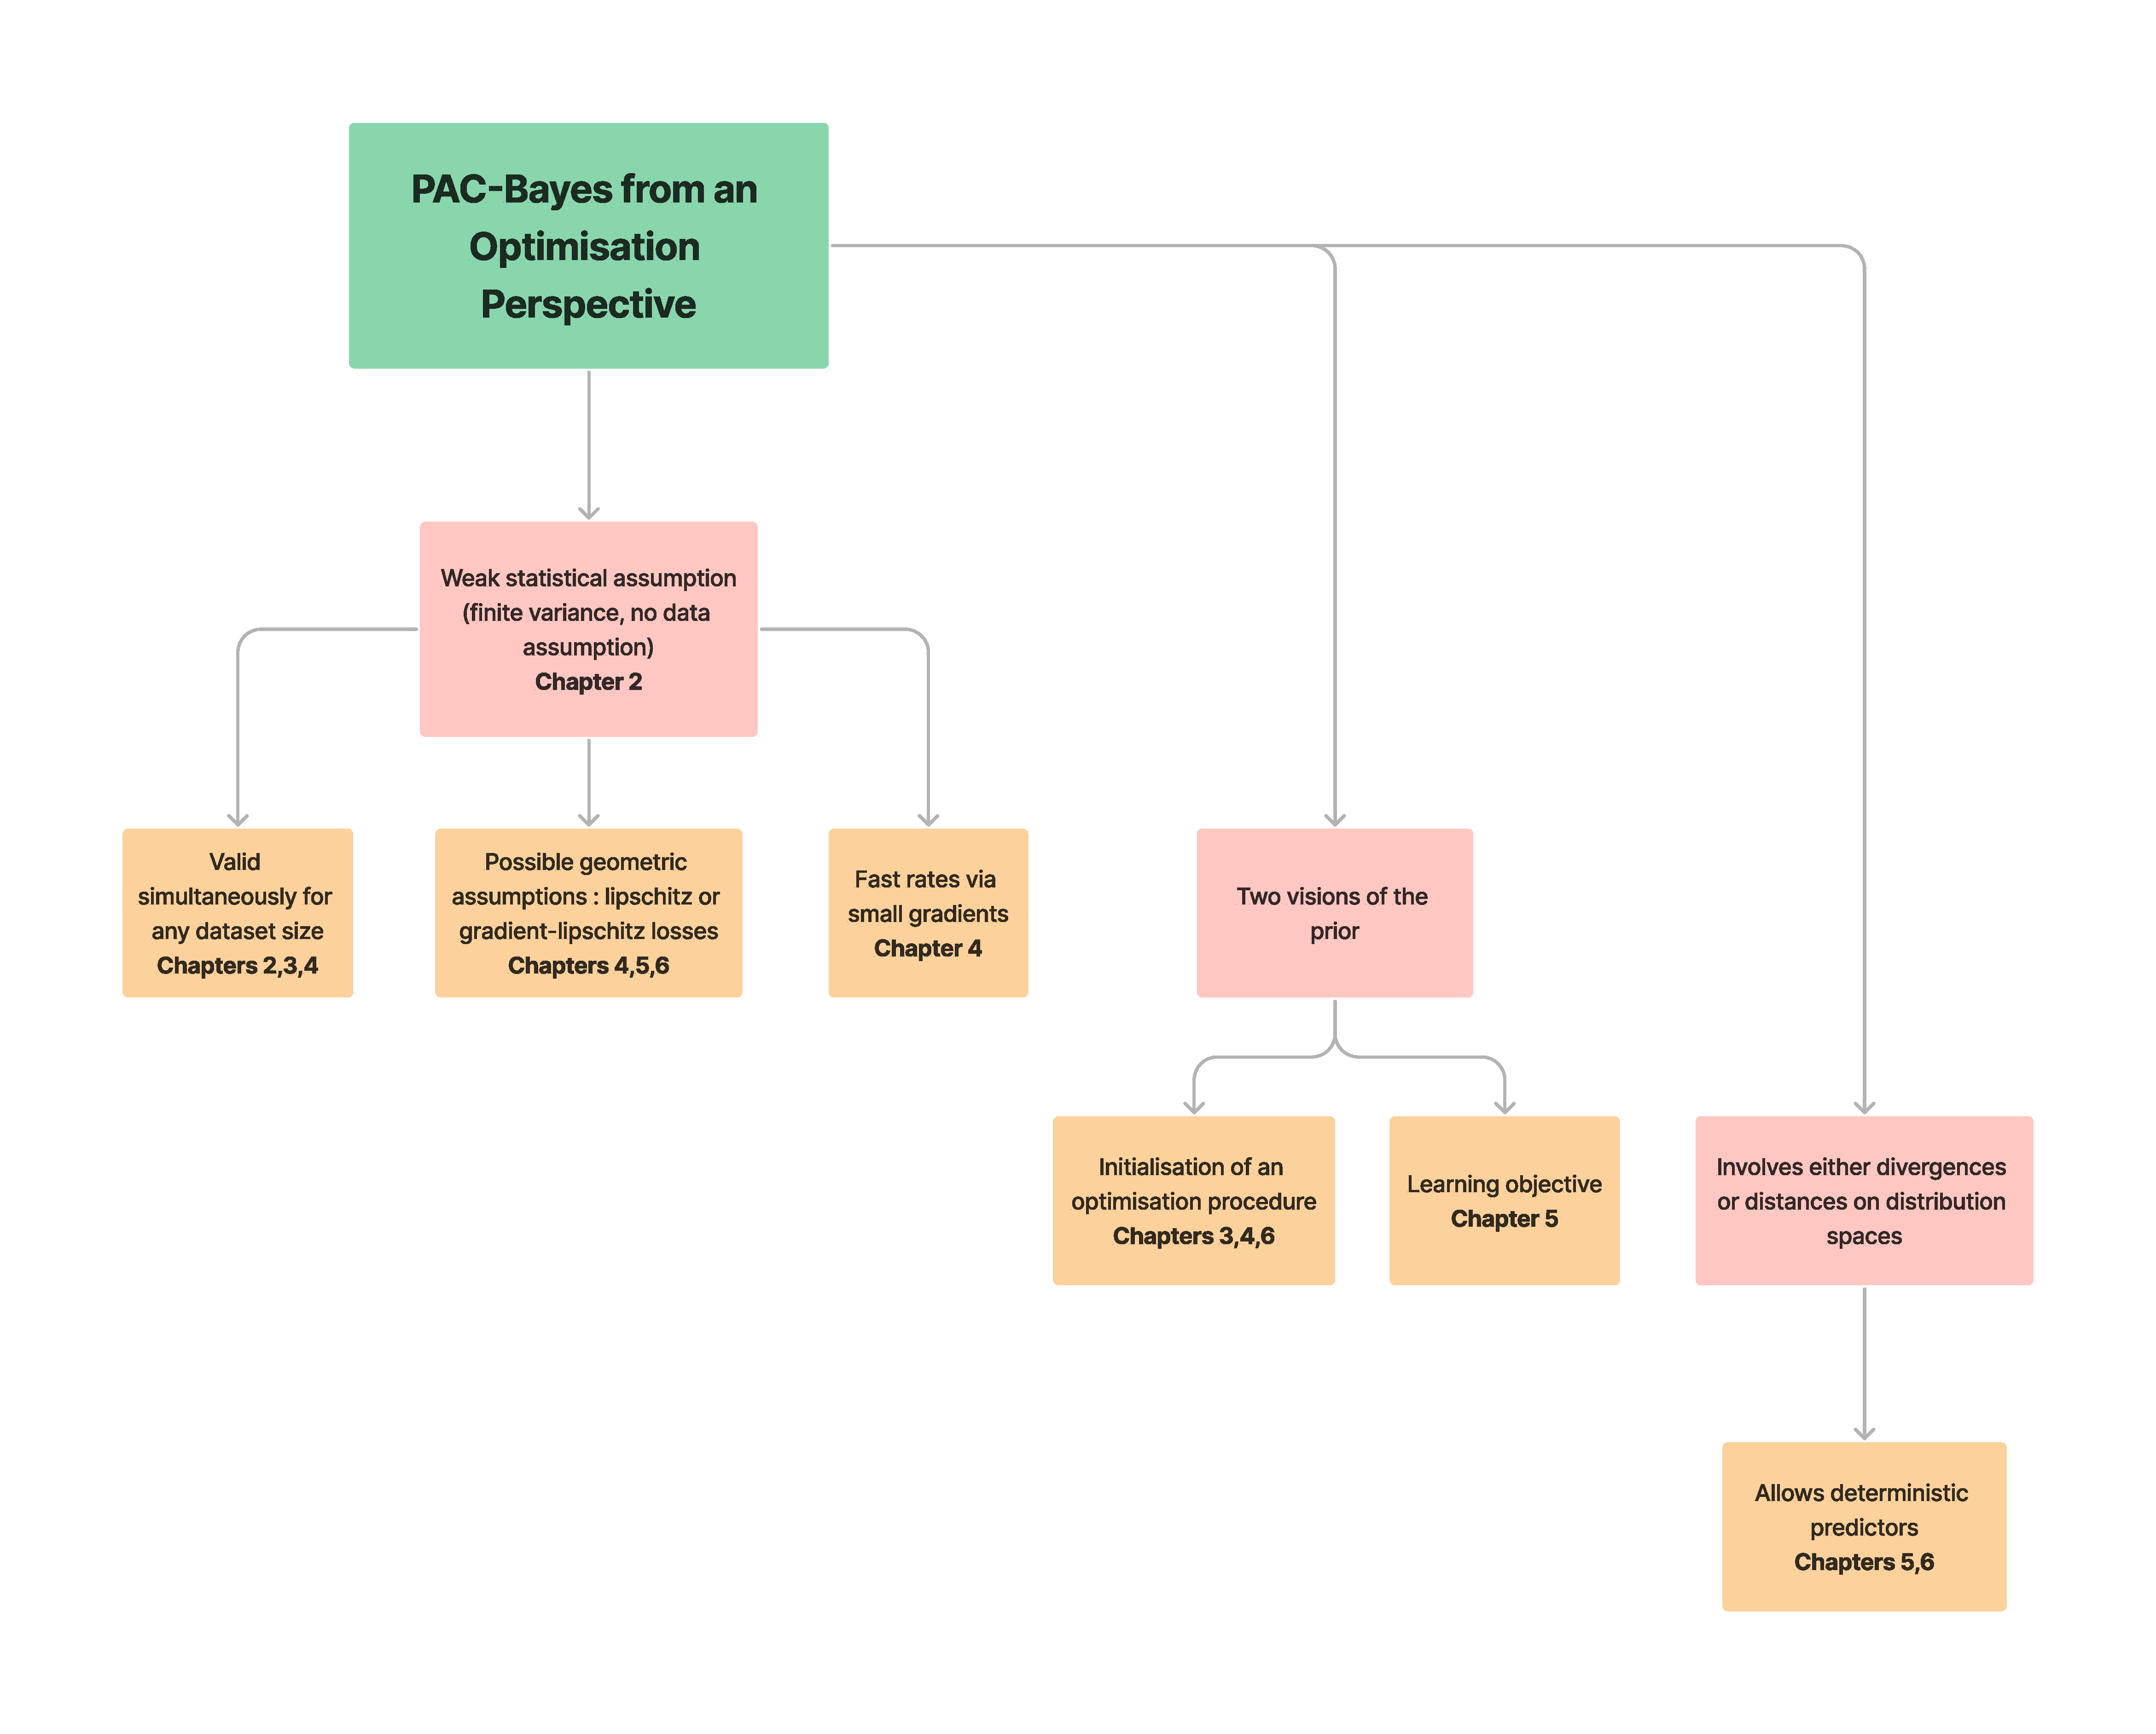
\includegraphics[width=1.0\linewidth]{chapter_1/recap-optim.pdf}
  \caption{Recap of the optimisation vision of PAC-Bayes and  where those views are exploited in the manuscript.}
  \label{fig: recap-optim}
\end{figure}


